
\section{View Points}
\label{sec:view_points} 

The 'View Points' tool of the Flight Deck displays existing view points, allows selection, stepping and editing of view points. 
Additionally, view points can be imported, removed and exported.

\begin{figure}[H]
    \hspace*{-2.5cm}
    
\includegraphics[width=19cm,frame]{figures/view_points.png}
  \caption{View Points Overview}
\end{figure}

At the top, a toolbar is shown. In the middle, a table showing all existing view points exists. At the bottom, general function buttons exist. \\

\subsection{View Point}

A view point is a point of interest in the data persisted in the database. It can have the following attributes:

\begin{center}
 \begin{table}[H]
  \begin{tabularx}{\textwidth}{ | l | X | }
    \hline
    \textbf{Key} & \textbf{Value Description} \\ \hline
    id & Identifier, as number \\ \hline
    type & Type, e.g. 'Short track', 'Extra track', 'Content deviation X'  \\ \hline
    status & Editable status, e.g. 'open', 'closed', 'todo' \\ \hline
    comment & Editable user comment \\ \hline
    text & Description text \\ \hline
    position\_latitude & Center position WGS-84 latitude \\ \hline
    position\_longitude & Center position WGS-84 longitude \\ \hline
    position\_window\_latitude & Geographic window size in WGS-84 latitude  \\ \hline
    position\_window\_longitude & Geographic window size in WGS-84 longitude  \\ \hline
    timestamp & Center timestamp in YYYY-mm-DD HH:MM:SSS.ZZZ  \\ \hline
    time\_window & Time window size \\ \hline
    data\_sources & Data sources and lines to be loaded \\ \hline
    data\_sources\_types & Data source types to be loaded \\ \hline
    filters & Filter configuration \\ \hline
    context\_variables & Context DBContent variables to be shown \\ \hline
    annotations & Displayable view annotations \\ \hline
\end{tabularx}
\end{table}
\end{center}
\ \\

Not all attributes are shown in the table, since some are more processing related than information relative to the user. \\

Also, additional attributes can be shown. If other additional attributes exist in the view point information, they are automatically shown in the table. For additional information please refer to \nameref{sec:view_points_custom_attributes}. \\

When a view point is selected, the dataset defined by the view point is loaded automatically and the active Views show the relevant data. Using the elements described in the following sections a user can quickly step through view points, assess the information shown and change status and comment information. \\

Please \textbf{note} that changes to view points are saved immediately to the database and no undo function exists.

\subsection{Toolbar}

\begin{table}[H]
  \center
  \begin{tabular}{ | l | l | l |}
    \hline
    \textbf{Icon} & \textbf{Text} &  \textbf{Description} \\ \hline
    \includegraphics[width=0.5cm,frame]{../../data/icons/up.png} & Select Previous [Up] & Steps to the previous view point \\ \hline
    \includegraphics[width=0.5cm,frame]{../../data/icons/not_recommended.png} & Set Selected Status Open [O] & Sets the current view point to status 'open' \\ \hline
    \includegraphics[width=0.5cm,frame]{../../data/icons/not_todo.png} & Set Selected Status Closed [C] & Sets the current view point to status 'closed' \\ \hline
    \includegraphics[width=0.5cm,frame]{../../data/icons/todo.png} & Set Selected Status ToDo [T] & Sets the current view point to status 'todo' \\ \hline
    \includegraphics[width=0.5cm,frame]{../../data/icons/comment.png} & Edit Comment [E] & Edits the current view points status \\ \hline
    \includegraphics[width=0.5cm,frame]{../../data/icons/down.png} & Select Next [Down] & Steps to the next view point \\ \hline
    & Edit Columns & Open menu for hiding/showing columns \\ \hline
    & Filter By Type & Opens menu for filtering based on type \\ \hline
    & Filter By Status & Opens menu for filtering based on status \\ \hline
  \end{tabular}
  \caption{Toolbar Actions}
\end{table}
\ \\

All of the actions can be triggered using the listed keyboard shortcut in the square brackets. Up/Down refers to the keyboard arrows.

\subsection{Table}

\begin{figure}[H]
    \hspace*{-2cm}
    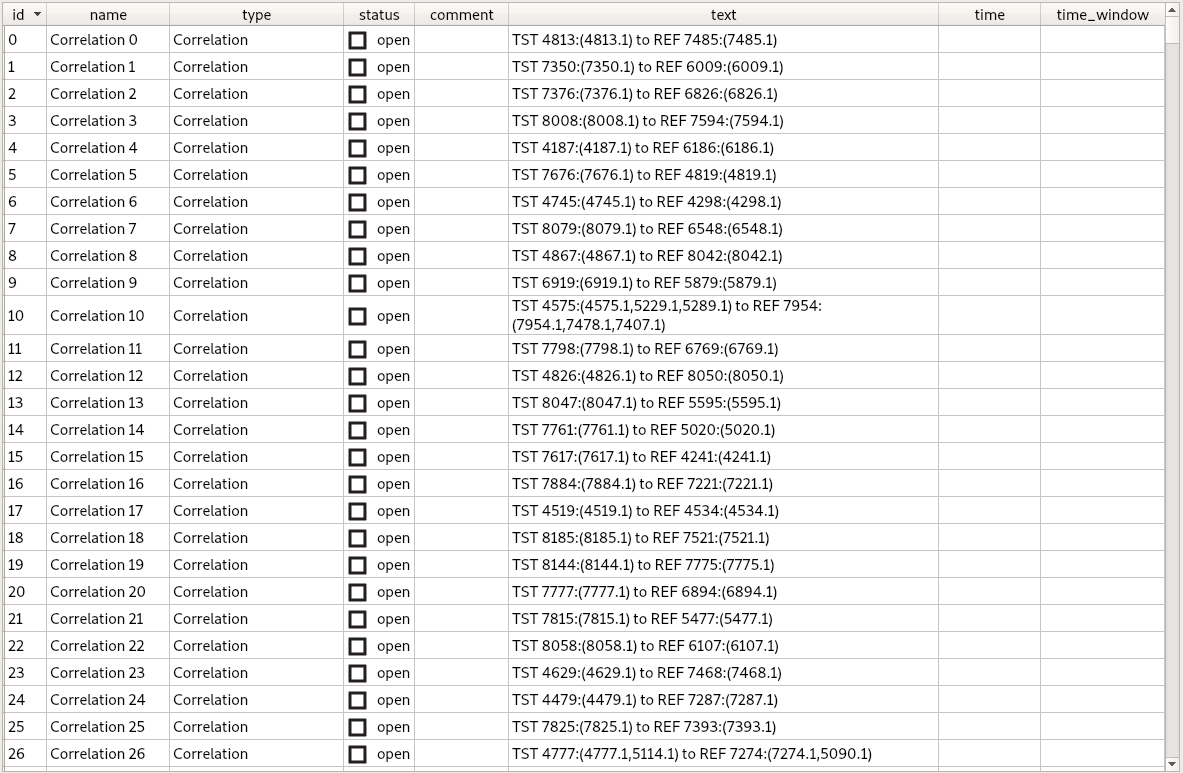
\includegraphics[width=18cm,frame]{figures/view_points_table.png}
  \caption{View Points Table}
\end{figure}

In the view points table, all view points are listed, each one in a seperate row. Columns can be used for ordering (simply click on the column name), and resized as wanted. \\

A click on a view point selects it, which highlights the row.

\begin{figure}[H]
    \hspace*{-2cm}
    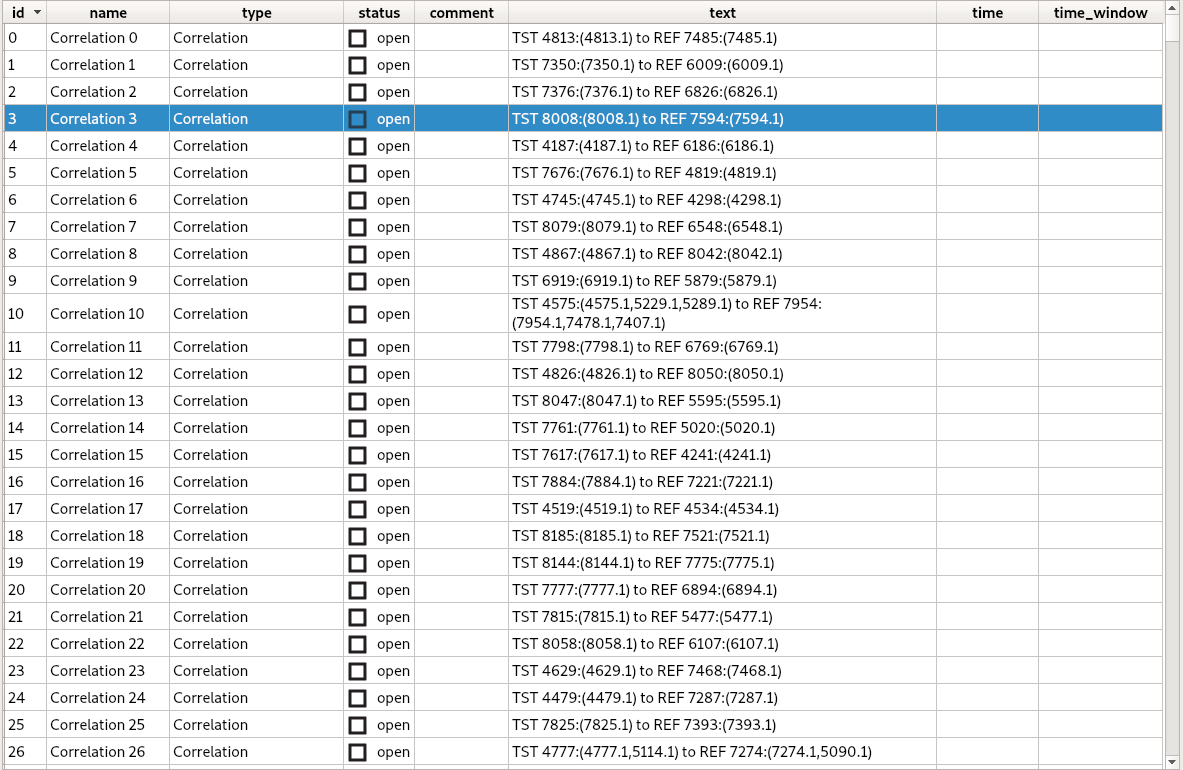
\includegraphics[width=18cm,frame]{figures/view_points_table_selected.png}
  \caption{View Points Table: Selected View Point}
\end{figure}

This automatically triggers loading of the data and display in the existing Views. \\

The status can only be set using the toolbar buttons or keyboard shortcuts, while editing the comment can also be triggered by a double-click on the respective cell.

\subsection{Re-Sorting Using Columns}

By clicking on a column, the View Points Table is sorted on the information in the column. Ascending/descending can be changed by clicking again on a column already used for sorting. \\

Per default, the table is sorted by the 'id' column.

\subsection{Showing/Hiding Columns}

Using the 'Edit Columns' button in the toolbar, unwanted columns can be hidden. Click on the button to activate the following menu:

\begin{figure}[H]
  \centering 
    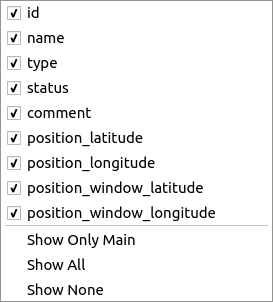
\includegraphics[width=6cm,frame]{figures/view_points_edit_columns.png}
  \caption{View Points: Edit Columns Menu}
\end{figure}

The following entries exist:

\begin{itemize}  
\item All Column names: With a checkbox to select/deselect which columns should be shown
\item Show Only Main: Only the first 4 columns are shown
\item Show All: All columns are shown
\item Show None: No columns are shown
\end{itemize}
\ \\

\subsection{Filtering Based on Type}

Using the 'Filter By Type' button in the toolbar, unwanted view points can be hidden. Click on the button to activate the following menu:

\begin{figure}[H]
  \centering 
    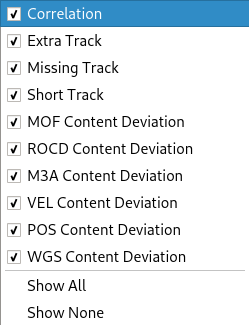
\includegraphics[width=5cm,frame]{figures/view_points_filter_type.png}
  \caption{View Points: Filter By Type Menu}
\end{figure}

The following entries exist:

\begin{itemize}  
\item All existing types: With a checkbox to select/deselect which should be shown
\item Show All: All types are shown
\item Show None: No types are shown
\end{itemize}
\ \\

\subsection{Filtering Based on Status}

Using the 'Filter By Status' button in the toolbar, unwanted view points can be hidden. Click on the button to activate the following menu:

\begin{figure}[H]
  \centering 
    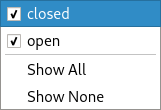
\includegraphics[width=4cm,frame]{figures/view_points_filter_status.png}
  \caption{View Points: Filter By Status Menu}
\end{figure}

The following entries exist:

\begin{itemize}  
\item All existing statuses: With a checkbox to select/deselect which should be shown
\item Show All: All types are shown
\item Show None: No types are shown
\end{itemize}
\ \\

\subsection{Function Buttons}

There exist 3 buttons for general functions:

\begin{itemize}  
\item Import: Imports a view point file selected by the user (only recommended if no view points are already defined)
\item Delete All: Deletes all existing view points
\item Export: Exports all existing view points as a view point file
\item Export PDF: Exports view points as a PDF file
\end{itemize}
\ \\

\subsection{Stepping View Points}

\subsection{Management Tab} 
When selecting a new view point, the information set 'data\_sources' and 'data\_sources\_types' attributes are used to select which DBContent is loaded. The 'filters' attribute to set the filter active flags and respective conditions. After that, a loading process is triggered. \\

\subsubsection{Data Selection}

When the loading process is finished, data is automatically selected using the 'time' and 'time\_window' attributes.

\subsubsection{Table View} 

\begin{figure}[H]
    \hspace*{-2cm}
    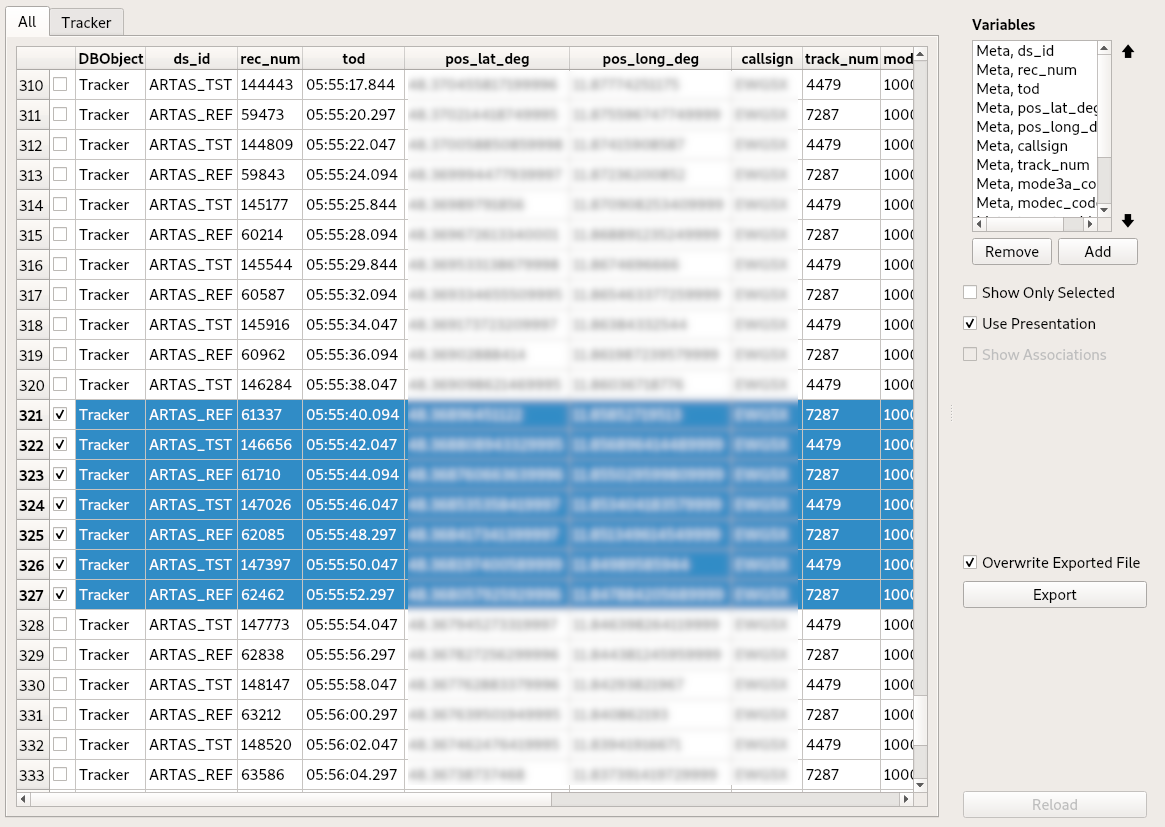
\includegraphics[width=18cm,frame]{figures/view_points_tableview_selected.png}
  \caption{View Points Table View: Selected View Point}
\end{figure}

In the Table View, the variables set in the 'context\_variables' attribute are added temporarily to the list of variables. Loaded data is presented as always. When the loading process is finished, selected data is highlighed.

\subsubsection{Geographic View}

\begin{figure}[H]
    \hspace*{-2cm}
    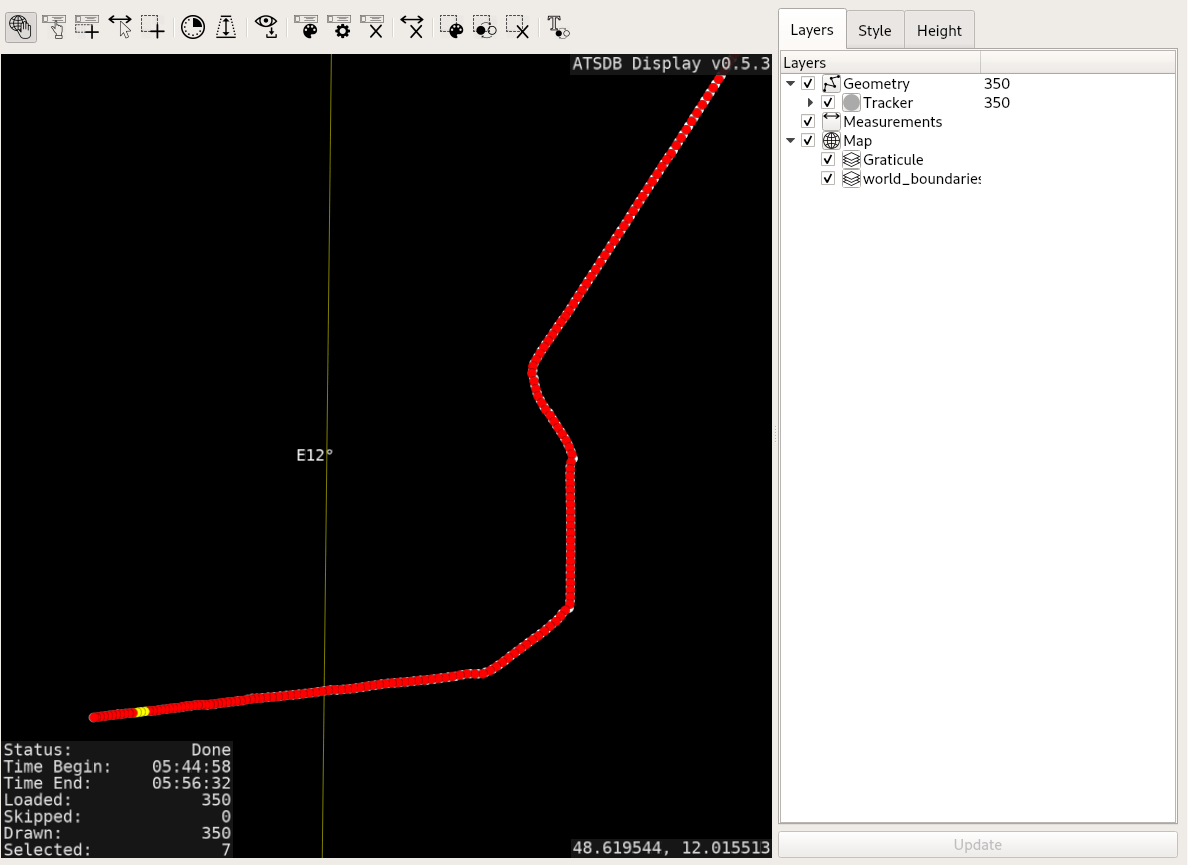
\includegraphics[width=18cm,frame]{figures/view_points_geoview_selected.png}
  \caption{View Points Geographic View: Selected View Point}
\end{figure}

Loaded data is presented as always and can be adapted to a users needs. After loading, the presented data is centered/zoomed according to the 'position\_latitude', 'position\_longitude', 'position\_window\_latitude', 'position\_window\_longitude' attributes. If these are not set, the center/zoom is adapted to encompass all of the loaded data. \\

Please \textbf{note} that using view points in 3D maps is currently not recommended, since the zoom-to-data function does not work well with small data geometry. If a view point is used with a 3D map, a warning is shown (only once per COMPASS usage, but ignored for subsequent usages).

\subsubsection{After Selection}

After data loading, the application can be used as in any other situation, therefore changing filters, adapting the Geographic View style or re-loading the dataset is possible.

\subsubsection{Assessment}

In the 'View Points' tab, after assessing the view point, a user can add a comment and change the status to annotate the view point with additional information. \\

After this e.g. the next view point can be selected.

\subsection{Exporting View Points to PDF}
\label{sec:view_points_export_pdf} 

Using the "Export PDF" button, a PDF can be generated. A PDF can only be generated if a Latex environment is installed on the workstation, as described in \nameref{sec:appendix_latex}. \\

Please note that:

\begin{itemize}  
\item Commonly the shown (filtered) View Points are exported, in the configured order
\item A Latex report file is generated, as well as View screenshots
\item To compile the Latex report into PDF a Latex environment (including the pdflatex application) must be installed, e.g. TeX Live (used by the author) and MikTeX (see \href{https://en.wikipedia.org/wiki/LaTeX}{Link})
\item All active views are included, so they should be configured in a suitable manner
\begin{itemize}  
\item A TableView is reported as the selected data, or the first 30 rows (if no data is selected), in a table.
\item An Geographic View is reported as a screenshot figure.
\end{itemize}
\end{itemize}
\ \\

\begin{figure}[H]
  \centering 
    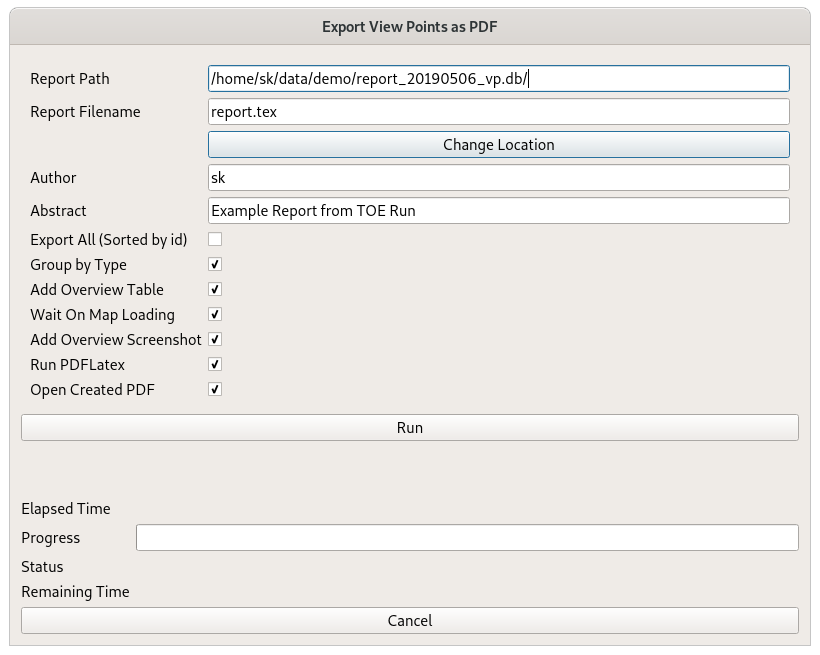
\includegraphics[width=14cm]{figures/view_points_export_pdf.png}
  \caption{View Points: Export PDF Dialog}
\end{figure}

At the top, the following configuration options exist:

\begin{itemize}  
\item Report Path: Directory to which the report will be written.
\item Report Filename: Filename of the report, to be created in the report path. File extension must be '.tex'.
\item Change Location: Button to set the report path and filename.
\item Author: Author string, is added to the first page of the report.
\item Abstract: Abstract string, is added to the first page of the report.
\item Export All (Sorted by id): Export all view points, sorted by id, ignoring the filtering and ordering in the View Point tab.
\item Group by Type: Creates sub-section for each type of View Point.
\item Add Overview Table: Creates table with an overview of all View Points in the beginning of the document. 
\item Wait on Map Loading: When Geographic View screenshots are created, some maps require downloading terrain from the Internet.  This option enables to wait on completion of such activities, to generate high-quality screenshots. Disable only when operating on cached maps without an Internet connection.
\item Add Overview Screenshot: Adds a preceding screenshot per Geographic View with an larger map overview and a data marker.
\item Run PDFLatex: Automatically runs the pdflatex compile process, immediately creating a PDF after finished export. Is disabled if command could not be found.
\item Open Created PDF: Automatically opens the created PDF. Is disabled if pdflatex command could not be found.
\end{itemize}
\ \\

The 'Run' button startes the export process. At the bottom, status information and a cancel button exists. \\

To run the export process, click the 'Run' button.

\begin{figure}[H]
  \centering 
    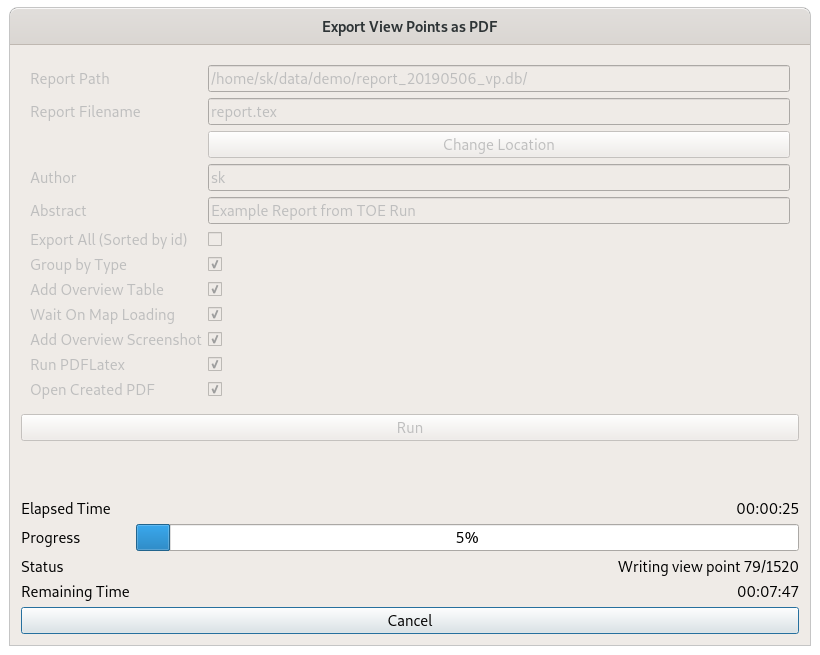
\includegraphics[width=14cm]{figures/view_points_export_pdf_status.png}
  \caption{View Points: Export PDF Dialog Status}
\end{figure}

If pdflatex is to be run, this is indicated in the 'Status' text, which might have to be run several times. For large documents this might take several minutes, this time not being included in the 'Remaining Time' estimate.

\begin{figure}[H]
  \centering 
    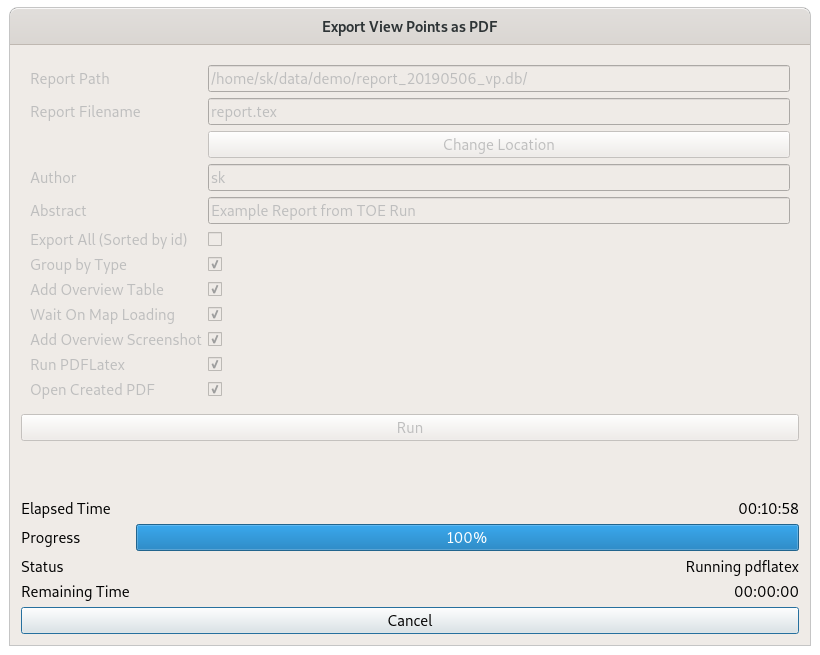
\includegraphics[width=14cm]{figures/view_points_export_pdf_status2.png}
  \caption{View Points: Export PDF Dialog Status: pdflatex}
\end{figure}

The export speed of course depends on the View Points, the number of Views, hardware etc. However, even exporting (somewhat unreasonable) 1500 View Points takes about only 15 minutes on the authors hardware, so it should be adequate for any reasonable use case. \\

If the export process was sucessful, a message is shown and the dialog is closed automatically. The report Latex file was written into the report directory, with screenshots in the 'screenshots' subfolder. If the respective options were set, a PDF was automatically generated and is opened using the default PDF application. \\

If a Latex error ocurred, a message box with the error message is shown. \\

Please note that the generated report can of course be edited by the user and re-generated using pdflatex, which allows for better customization options (adding e.g. details, corporate identity etc.).

